                %%%%%%%%%%%%%%%%%%%%%%%%%%%%%%%%%%%%%%%%%
% Beamer Presentation       Hola
% LaTeX Template
% Version 1.0 (10/11/12)
%
% This template has been downloaded from:
% http://www.LaTeXTemplates.com
%
% License:
% CC BY-NC-SA 3.0 (http://creativecommons.org/licenses/by-nc-sa/3.0/)
%
%%%%%%%%%%%%%%%%%%%%%%%%%%%%%%%%%%%%%%%%%

%----------------------------------------------------------------------------------------
%   PACKAGES AND THEMES
%----------------------------------------------------------------------------------------

\documentclass{beamer}

\mode<presentation> {

% The Beamer class comes with a number of default slide themes
% which change the colors and layouts of slides. Below this is a list
% of all the themes, uncomment each in turn to see what they look like.

%\usetheme{default}
%\usetheme{AnnArbor}
%\usetheme{Antibes}
%\usetheme{Bergen}
%\usetheme{Berkeley}
%\usetheme{Berlin}
%\usetheme{Boadilla}
\usetheme{CambridgeUS} %si
%\usetheme{Copenhagen}
%\usetheme{Darmstadt}
%\usetheme{Dresden}
%\usetheme{Frankfurt}
%\usetheme{Goettingen}
%\usetheme{Hannover}
%\usetheme{Ilmenau}
%\usetheme{JuanLesPins}
%\usetheme{Luebeck}
%\usetheme{Madrid}
%\usetheme{Malmoe}
%\usetheme{Marburg}
%\usetheme{Montpellier}
%\usetheme{PaloAlto}
%\usetheme{Pittsburgh}
%\usetheme{Rochester}
%\usetheme{Singapore}
%\usetheme{Szeged}
%\usetheme{Warsaw}

% As well as themes, the Beamer class has a number of color themes
% for any slide theme. Uncomment each of these in turn to see how it
% changes the colors of your current slide theme.

%\usecolortheme{albatross}
%\usecolortheme{beaver}
%\usecolortheme{beetle}
%\usecolortheme{crane}
\usecolortheme{dolphin}
%\usecolortheme{dove}
%\usecolortheme{fly}
%\usecolortheme{lily}
%\usecolortheme{orchid}
%\usecolortheme{rose}
%\usecolortheme{seagull}
%\usecolortheme{seahorse}
%\usecolortheme{whale}
%\usecolortheme{wolverine}

%\setbeamertemplate{footline} % To remove the footer line in all slides uncomment this line
%\setbeamertemplate{footline}[page number] % To replace the footer line in all slides with a simple slide count uncomment this line

%\setbeamertemplate{navigation symbols}{} % To remove the navigation symbols from the bottom of all slides uncomment this line
}

\usepackage{graphicx} % Allows including images
\usepackage{booktabs} % Allows the use of \toprule, \midrule and \bottomrule in tables
\usepackage{ragged2e}
\usepackage[spanish]{babel}
\graphicspath{{Pictures/}}
\usepackage[utf8]{inputenc}

\usepackage{hyperref}
%----------------------------------------------------------------------------------------
%   TITLE PAGE
%----------------------------------------------------------------------------------------

\title[Trafico]{Tráfico} % The short title appears at the bottom of every slide, the full title is only on the title page

\author{Luis Olaya} % Your name
\institute[UPA] % Your institution as it will appear on the bottom of every slide, may be shorthand to save space
{
Universidad de Pamplona \\ % Your institution for the title page

}
\date{\today} % Date, can be changed to a custom date

\begin{document}
\justifying 

\begin{frame}
\titlepage % Print the title page as the first slide
\end{frame}

\begin{frame}
	\frametitle{Contenido} % Table of contents slide, comment this block out to remove it
	\tableofcontents % Throughout your presentation, if you choose to use \section{} and \subsection{} commands, these will automatically be printed on this slide as an overview of your presentation
\end{frame}

\section{Introducción} % Sections can be created in order to organize your presentation into discrete blocks, all sections and subsections are automatically printed in the table of contents as an overview of the talk
%------------------------------------------------

%\subsection{Subsection Example} % A subsection can be created just before a set of slides with a common theme to further break down your presentation into chunks

\begin{frame}
	\frametitle{Introducción}
	
	\justifying 
	Hemos  analizado el articulo de titulo [Medición de la complejidad de semáforos auto-organizables] en el cual se da el analisis del funcionamiento de los semaforos a partir de una simulación en NetLogo en donde se nota el comportamiento de los carros ó [turtles] al momento de llegar a los semaforos en las intersecciones, y adicional se han investigado software basados en c++ para la simulacion de redes. 
	
	\href{https://es.wikipedia.org/wiki/IEEE_802.15}{Hipervinculo}
\end{frame}

\section{Contextualización} 
\subsection{Métodos}
%
\begin{frame}
	\frametitle{Artículo}
	
	\begin{columns}[c] % The "c" option specifies centered vertical alignment while the "t" option is used for top vertical alignment
		% 	
		\column{.4\textwidth} % Left column and width
		\begin{itemize}
			\item Metodo de onda verde
			\item Metodo de auto-organización
		\end{itemize}
		\column{.4\textwidth} % Right column and width
		\begin{figure}
			\label{[fig01]}
			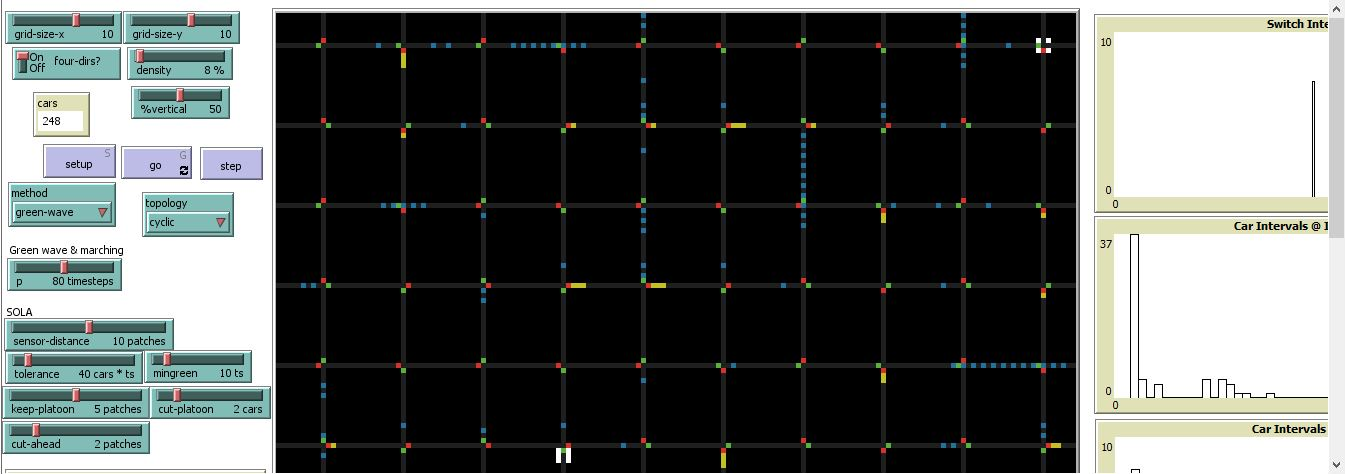
\includegraphics[scale=0.2]{net.JPG}
		\end{figure}
		
	\end{columns}
	
	
	
\end{frame}
%
%%------------------------------------------------
%

\begin{frame}
	\frametitle{Método de onda verde}
	Es el más utilizado en grandes ciudades para la coordinación de semáforos. Estos semáforos tienen el mismo período y la compensación. Una vez que los vehículos consiguen una luz verde, ellos no deberían conseguir ninguna luz en rojo.\\
	Además, si los vehículos no van en la velocidad esperada (como esto es el caso cuando el cambio de densidad), entonces los vehículos no serán capaces de ir en la velocidad de la onda verde y tendrán que pararse.
	
	
	%\begin{block}{Clustering}
	%	Los datos de entrada pueden ser agrupados en “clusters” y el sistema al procesar los datos debe de encontrar los centros de esos clusters.
	%\end{block}
	%
\end{frame}
%
%%------------------------------------------------
%

\begin{frame}
	\frametitle{Método de auto-organización}
	
	Se propuso en el artículo el método de auto organización para la coordinación de luz de tráfico:\\
	\begin{itemize}
		\justifying 
		\item En cada marca, añada a un contador el número de acercamiento de vehículos o espera en una luz roja dentro de la distancia d. Cuando este contador exceda un umbral n, cambie la luz. Siempre que los interruptores de luz, reinicio el contador a cero.
		\item Las luces deben permanecer verdes durante un tiempo mínimo u.
		\item Si unos vehículos (m o menos, pero más de cero) se deja cruzar en luz verde en distancia r corto, no cambie la luz
	\end{itemize}
	
	%4. 
	%5. 
	%6. 
	
	%
	
	%
	%\begin{block}{Reducción de Dimensionalidad: }
	%	Los datos de entrada deben de ser agrupados en un subespacio con una dimensionalidad más baja que la dimensionalidad de los datos.
	%\end{block}
	%
	%\begin{block}{Extracción de Características:  }
	%	El sistema tiene que extraer características de los datos de entrada (supone casi siempre una reducción de la dimensionalidad).
	%\end{block}
	%
\end{frame}
\begin{frame}
	\frametitle{Método de auto-organización}
	
	
	\begin{itemize}
		\justifying 
		\item Si ningún vehículo se acerca a una luz verde dentro de una distancia d, y por lo menos un vehículo se acerca a la luz roja dentro de una distancia d, a continuación, cambie la luz.
		\item Si hay un vehículo parado en la calle una distancia corta e más allá de un semáforo verde, entonces cambie la luz. 
		\item Si hay un vehículo parado en ambas direcciones a una distancia corta e más allá de la intersección, entonces cambie ambas luces a rojo. Una vez que una de las direcciones es libre, restaure la luz verde en esa dirección. 
	\end{itemize}
\end{frame}
\subsection{Netlogo}
%%------------------------------------------------
%
\begin{frame}
	\frametitle{Netlogo}
	Es una plataforma para el desarrollo y estudio de sistemas multiagente, es un software libre, utiliza turtles (tortugas)  y patches (parches) para la interacción en el sistema.\\ 
	
	\begin{block}{Agentes: }
		Un agente es una entidad capaz de percibir las condiciones exteriores de entorno donde habita e interiores a sí mismo para realizar acciones de forma independiente y autónoma.
	\end{block}
	
	
\end{frame}
%
%%------------------------------------------------
%
\begin{frame}
	\frametitle{Netlogo}
	Un agente presenta características como:
	\begin{itemize}
		\item \textcolor{blue}{Autonomía:} capaz de operar sin intervención directa de un ente externo
		\item \textcolor{blue}{Reactividad:} capaz de responder a cambios que ocurren en el entorno
		\item \textcolor{blue}{Pro-actividad:} capaz de iniciar acciones como respuesta a estados internos
		\item \textcolor{blue}{Habilidad social:} capaz de interactuar con otros agentes.
	\end{itemize}
	
\end{frame}

\begin{frame}
	\frametitle{Netlogo}
	\begin{figure}
		\label{[fig02]}
		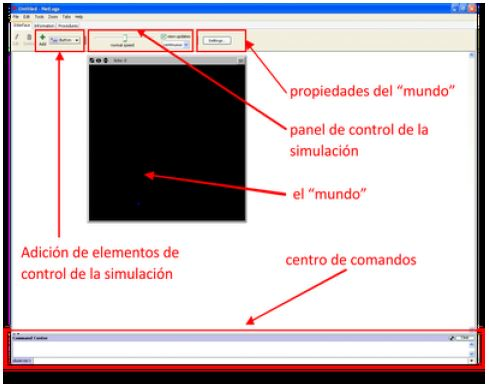
\includegraphics[scale=0.7]{partes_Netlogo.JPG}
	\end{figure}
\end{frame}
\subsection{C++ Simuladores }

%
%%------------------------------------------------
%\section{Características}
%%------------------------------------------------
%
\begin{frame}[fragile] % Need to use the fragile option when verbatim is used in the slide
	
	\frametitle{Simuladores en C++}
	\textcolor{blue}{OMNeT++}
	\begin{itemize}
		\item Es un paquete de simulación de eventos discretos basado en C++.
		\item Su objetivo es simular redes computacionales y otros sistemas distribuidos. 
		\item Es completamente programable y modular.
		\item Permite simulaciones a gran escala formadas por modelos de componentes reutilizables. 
		\item Permite una fácil trazabilidad y depuración de los modelos de simulación a través de su interface gráfica de usuario que muestra los gráficos de la red y animaciones del flujo de los mensajes.
		\item Permite al usuario modificar variables y objetos sin que éste deba entrar en términos de programación del modelo.
		\item Es de código abierto y libre para uso académico y sin ánimo de lucro. Su versión comercial es OMNEST (desarrollada por Omnest Global, Inc).
		
	\end{itemize}
	
\end{frame}
%
%%------------------------------------------------
%
\begin{frame}
	\frametitle{Simuladores en C++}
	\textcolor{blue}{Network Simulator 2 (NS – 2)}
	\vspace{0.5cm}
	\begin{itemize}
		\item Utiliza simulaciones de eventos discretos y que está pensado para el desarrollo de redes con un gran nivel de detalle. 
		\item Es de código abierto y está enfocado a la investigación.
		\item El lenguaje que utiliza es C++ y OTcl (Versión orientada a objetos del lenguaje Tcl).
		\item NS – 2 puede simular una gran variedad de protocolos de cualquier capa del modelo OSI.
		\item Implementa todo tipo de redes, redes cableadas, inalámbricas, satelitales, etc.
	\end{itemize}
	
	
\end{frame}
\end{document}
